\subsection{Sickness}
\begin{frame}[t]{Sickness [JH]p19-21, [RH]p11-13 }
The question was about a sick person, \textsl{"whether he would be freed from his sickness, or whether he would die"} \\
\vspace{0.25cm}
\begin{columns}[T, onlytextwidth]
\column{0.5\textwidth}
\Mercury\ (L1)  Void of Course in the 8th signifies \textsl{"the strength of pain and the fear of death"} as does \Mars\ (L8) in the 10th aspecting the 1st who signifies \textsl{"the strength of pain and the loss of hope". } \\

\vspace{0.2cm}
\Mercury (L1) is Void of Course, does not aspect the 1st, and is not first to leave his sign. \\

\vspace{0.2cm}
The \Moon\ is also Void of Course but she is \Trine\ the 1st House and she is the first to enter a new sign so she is the stronger significator. \\

\vspace{0.2cm}
The two significators of the querent, both VOC, signified \textsl{"a prolongation of the sickness"} and its severity.\\


\column{0.5\textwidth}
\begin{center}
\vspace{-0.75cm}
{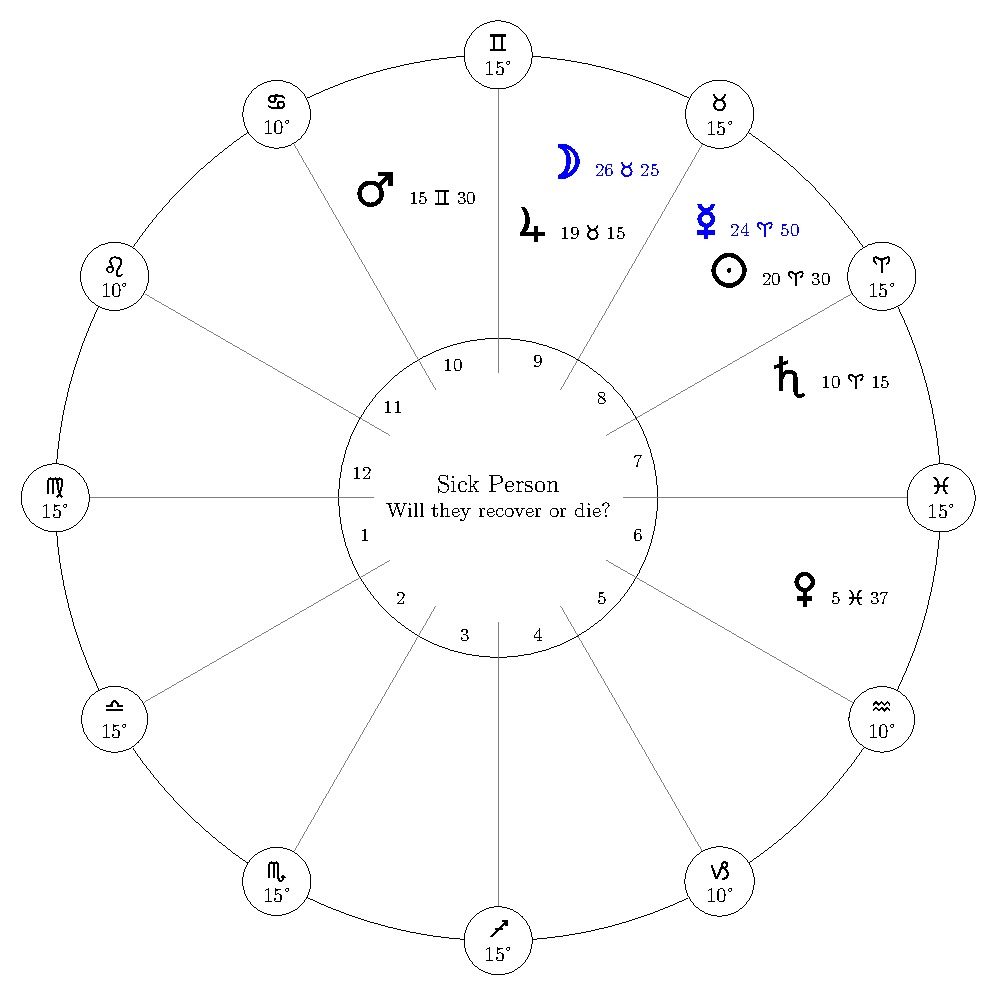
\includegraphics[width=0.9\textwidth]{charts/21-chart-sickness}} \\
\end{center}
\end{columns}

\end{frame}
% ------------------------------------------------------------
\begin{frame}[t]{Sickness Continued}
\begin{columns}[T, onlytextwidth]
\column{0.5\textwidth}
We look at the \Moon, the stronger significator, first. \\
\vspace{0.2cm}
\textbf{\Moon\ in \Taurus\ \Trine\ 1st House} enters \Gemini \\
$\Rightarrow$ \Square\ \Venus\ (in 6th, sickness)  \\
\Venus\ $\Rightarrow$ \Sextile\ \Jupiter, MR by domicile \\

\vspace{0.2cm}
As \Jupiter\ cannot join with any other planet\footnotemark[1], he ends the disposition and becomes the final authority over the matter and so determines the final outcome.

\vspace{0.2cm}
After examining the \Moon\ committing her disposition, Masha'allah looks at \Mercury\ (L1) as sharing in the matter and finds it confirms what the \Moon\ signified.



\column{0.5\textwidth}
\begin{center}
{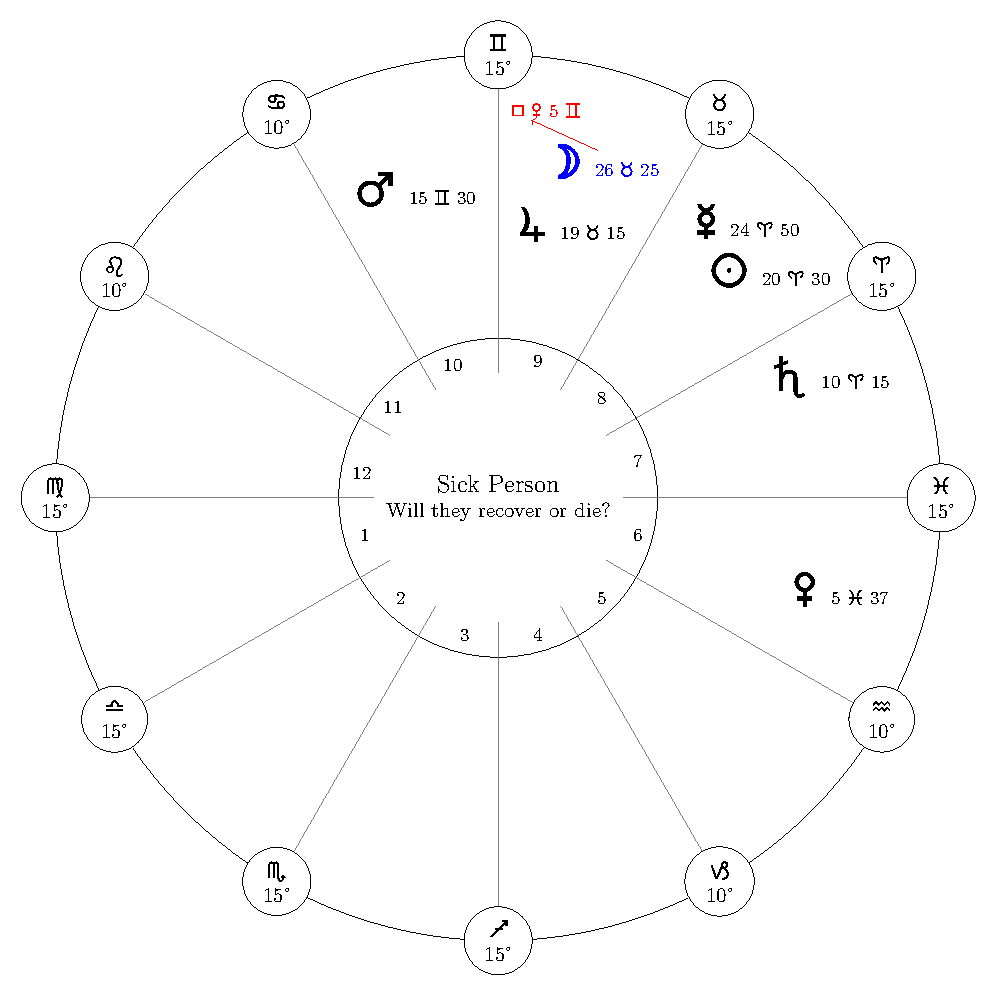
\includegraphics[width=0.9\textwidth]{charts/21a-chart-sickness}} \\
\vspace{-0.2cm}
\end{center}
\end{columns}
\footnotetext[1]{He can only apply to \Saturn\ and he is already separated from him.}
\end{frame}
% ------------------------------------------------------------
\begin{frame}[t]{Sickness Continued}
\begin{columns}[T, onlytextwidth]
\column{0.5\textwidth}

\textbf{\Mercury\ in \Aries\ Void of Course} $\Rightarrow$ \Taurus \\
$\Rightarrow$ \Sextile\ \Venus\ in \Taurus\ accepts his disposition\footnotemark[1] \\
\Venus\ $\Rightarrow$ \Sextile\ \Jupiter\ in \Taurus\, MR by domicile \\
And again, \Jupiter\ is the end of the disposition chain, supporting what the \Moon\ indicated.
\vspace{0.2cm}

\Jupiter, a benefic, as the final arbiter of the disposition promises "health and quiet" and the end of the illness after a prolonged period (due to the VOC's) but we are told that from the time of \Venus\ accepting the \Moon's disposition to her (\Venus's) joining with \Jupiter\ by \Sextile, the person would have gradually strengthened, with the illness leaving him completely once \Venus\ separates from \Jupiter\ by one minute.

\column{0.5\textwidth}
\begin{center}
{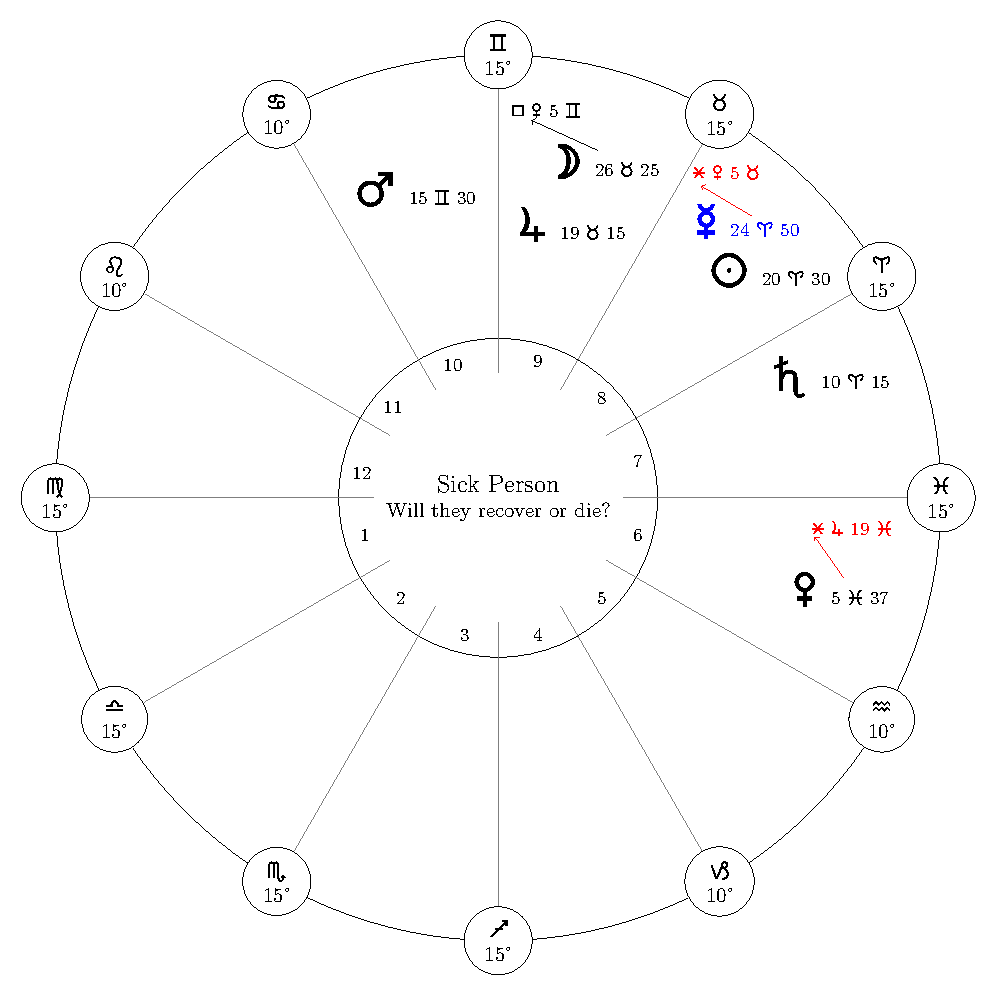
\includegraphics[width=0.9\textwidth]{charts/21b-chart-sickness}} \\
\vspace{-0.2cm}
\end{center}
\end{columns}
\footnotetext[1]{Sahl's mode 14.2, \textsl{Strength of the Planets}, says a planet in dignity can effectively accept a disposition; here it appears to apply to the location of the aspect but it could also apply because \Venus\ has dignity in her place, in \Pisces.}
\end{frame}
% -------------------------------------------------------------------------
\begin{frame}[t]{Sickness (Alternative Scenarios)}
The significator of the matter being asked about (death) is actually \Mars\ as the ruler of the 8th. Masha'allah does list a \Mars\ connection as an alternative scenario, saying such a connection would have meant death for the querent as \Mars's is L8 and does not receive \Venus\ in \Pisces. However, as neither L1 nor the \Moon\ joined to \Mars, the person did not die; although they had a severe illness (\Venus, while not the ruler of the 6th, is in the 6th of sickness). (\textbf{Note:} the \Moon, as the main significator of the querent, is averse to (\Semisextile) \Mars.)\\

\vspace{0.2cm}
He also goes on to warn that had the \Moon\ joined with the \Sun, as he is not L1, he can destroy by combustion if he does not receive the planet, and this also applies to his \Square\ or \Opposition. [JH p23.]\footnotemark[1]

\footnotetext[1]{I've seen this before as a planet being protected from combustion if they are in their own signs; here, the \Moon\ is in her Exaltation but we are told she has to be in the \Sun's signs (\Leo\ or \Aries) to be protected from combustion.}
\end{frame}